\documentclass[titlepage,a4paper,12pt]{article}
% Indica el estilo que se va a usar para todo el documento.
% Parámetros:
% a4paper, letterpaper, a5paper, …
% landscape: Apaisado
% titlepage: Hace que el tıtulo y el resumen queden en una página aparte. El resumen se indica con la instrucción \abstract{..}
% 10pt, 11pt, 12pt, … Tamaño de la letra.
% twoside, oneside. Simple o doble faz.
% twocolumn. Texto a dos columnas.
%
% Clases de documentos:
% article: Informes pequeños, trabajos prácticos.
% report: Informes largos, tesis, guiones. Tiene capítulos y apartados.
% book
% slide: Diapositivas

%%%%%%%%%%%%%%%%%%%%%%%%%%%%%%%%
% Paquetes
%%%%%%%%%%%%%%%%%%%%%%%%%%%%%%%%
\usepackage{color} % Paquete para darle color a la sintaxis del codigo fuente.

% Establece los márgenes de la hoja, aunque los margenes por defecto son bastante buenos.
\usepackage[top=2cm, bottom=2cm, left=2cm, right=2cm]{geometry} 

\usepackage{latexsym} % Este paquete permite usar simbolos especiales, no relacionados con la matemática, como  \Join o \Box
\usepackage{verbatim} % Para escribir codigo fuente.
\usepackage{amsmath} % La gran mayoría de los simbolos matemáticos
\usepackage{amssymb} % Algunos pocos símbolos matemáticos más raros, como \digamma
\usepackage{siunitx} % Notación exponencial
\usepackage{pdfpages} % Importar PDF

\usepackage[spanish]{babel} % Definimos el documento como que esta en español.

\usepackage[utf8]{inputenx} % Este paquete permite usar los acentos y eñes directamente en el texto.

\usepackage{graphicx} % Para usar imagenes
\usepackage{float}
\usepackage{courier}
\usepackage{listings} % Paquete para importar código fuente.

% Con esta instrucción definimos el interlineado. Por defecto es 1.
\linespread{1}

% Con esta instrucción obtenemos el número de página en el pie y una cabecera con el nombre de la sección (o con la sección en las páginas pares y la subsección en las impares si hemos indicado la opción twoside en el comando documenclass).
%\pagestyle{headings}

% Pero también está la instrucción \pagestyle{myheadings}, que pone el número de página al pie y en la cabecera pone el texto especificado por los comandos ``markboth{...}{...}'' y ``markright{...}''.
\pagestyle{myheadings}
%\markboth{Encabezado izquierdo}{Encabezado derecho} % Para doble faz
\markright{Trabajo Práctico Final: Dune 2000} % Para una carilla.

% Si no hemos especificado la opción twoside, todas las páginas se consideran derechas. Podemos cambiar el estilo de la página en curso mediante \thispagestyle. Por ejemplo, si queremos que la página en curso no tenga número escribimos \thispagestyle{empty} en el cuerpo del documeento.

%%%%%%%%%%%%%%%%%%%%%%%%%%%%%%%%
% Portada
%%%%%%%%%%%%%%%%%%%%%%%%%%%%%%%%

% En la instrucción \title{..}, se escribe el título del documento.
\title{ Trabajo Práctico Final: Dune 2000 \\ 
 \large{Informe Técnico}}

\author{Alvarez Juliá, Santiago \and Iglesias, Matias \and Sportelli Castro, Luciano}

% Aquí podemos escribir la fecha de realización del trabajo práctico. La fecha actual se escribe con \today. Si no se quiere incluir la fecha, dejar la instrucción en blanco.
\date{ \today }

%%%%%%%%%%%%%%%%%%%%%%%%%%%%%%%%%%%%%%%%%%%
% AQUI COMENZAMOS EL DOCUMENTO
%%%%%%%%%%%%%%%%%%%%%%%%%%%%%%%%%%%%%%%%%%%

\begin{document}

%Lo primero que hacemos es crear el titulo.
\maketitle

%Creamos los indices que sean necesarios.
\tableofcontents %Índice general
%\listoffigures %Indice de imágenes
%\listoftables %Indice de tablas

\newpage
\section{Introducción}
Para este trabajo práctico se desarrolló un clon del juego Dune 2000, producido por Westwood Studios en el año 1998. Se trata de un juego de estrategia multijugador en el cual se debe construir un ejército y vencer a sus oponentes destruyendo sus correspondientes edificios y tropas.
Cada jugador debe explorar el terreno de juego y recolectar especia melange que puede ser intercambiada por dinero para construir nuevos edificios que, a su vez, le habilitaran el entrenamiento de distintos tipos de tropas.

El clon realizado del juego espera ser una versión moderna y reducida del juego original. Durante el desarrollo del mismo se confeccionaron tres aplicaciones: el cliente de juego, encargado de interactuar con el jugador y mostrarle la interfaz del juego; el servidor del juego, encargado de administrar las partidas multijugador a través de la red y el editor de mapas que permite crear nuevos mapas de juego.

\section{Cliente}
El cliente del juego fue desarrollado en Qt5 y SDL 2.0. El mismo se compone de dos partes, el lanzador del juego, realizado enteramente en Qt5, que permite conectarse a un servidor, unirse o crear una sala de juego y luego iniciar el juego; y juego en sí, desarrollado en SDL.

\subsection{Arquitectura}
El juego se dividió en tres secciones: el área del juego, es decir, el terreno, las unidades y edificios; la interfaz de interacción con el usuario, en adelante el HUD; y la interfaz de conexión con el servidor.

Las primeras dos secciones son las encargadas de renderizar todos los elementos visuales en pantalla y atender los comandos que ingresa el usuario, por teclado o mouse, mientras que la última sección se encarga de recibir los eventos del servidor y actualizar la representación interna del modelo de juego de forma acorde.

Para la renderización de elementos se encapsuló la biblioteca SDL en las clases Ventana, Sonido y Textura. Todos los elementos se renderizan haciendo uso de la ventana y una o más texturas. En particular el área de juego se apoya en un elemento gráfico más, la cámara, que permite determinar que sección del terreno se está renderizando en este momento.

\subsubsection{Tropas y edificios}
Para el modelo gráfico de tropas y edificios se decidió implementar un diseño basado en prototipos. El mismo nos permitió tener menos clases, evitar la herencia y además tener más flexibilidad a la hora de ultimar detalles cómo el posicionamiento de los sprites, ya que tomamos la decisión de bajar esta información a archivos de datos. Tanto las tropas como los edificios cargan su modelo de datos desde archivos en formato JSON.

\subsubsection{Área de juego}
El área de juego es el componente central del cliente y está conformada por cuatro entidades que representan en conjunto la partida. La primer entidad es el Juego en sí, que reúne a las otras tres entidades y mantiene información sobre el juego del jugador a quién está representando, tales como la energía o el dinero.
Las siguientes entidades son infraestructura y ejército, que se encargan de administrar los edificios y las tropas de todos los jugadores en la partida.
Por último pero no menos importante está el terreno de juego. El terreno es un elemento central en este juego ya que es el encargado de detectar las interacciones entre elementos. 

El área de juego tiene una cámara que permite renderizar una sección del mismo y moverse sobre el terreno según sea necesario. 

\subsubsection{Visualización Head-Up}
Para la implementación del HUD se decidió utilizar un diseño basado en Widgets. Este diseño si bien no es sencillo de implementar, una vez resuelto permitió tener un sistema de eventos mucho más sencillo, mucha más movilidad a la hora de diseñar el HUD en sí y simplificar el problema de las dimensiones variables de la ventana. Con el diseño basado en Widgets, al correr el cliente en modo ventana o en modo pantalla completa el mismo se ajusta automáticamente según el espacio disponible.

La implementación de eventos en los widgets se hizo de forma directa utilizando herencia.

\subsection{Renderizado}
El renderizado de la ventana del cliente se realizó utilizando SDL2. Para esto se realizó un encapsulamiento de los subsistemas de SDL que permitieron abstraer el renderizado del juego de la biblioteca utilizada.

Todo el cliente utiliza texturas para el renderizado lo que implica que la mayor parte del trabajo se realiza directamente sobre la placa de video. Sin embargo, las texturas tienen una fuerte dependencia respecto del contexto de renderizado lo cual trajo algunos problemas respecto del encapsulamiento\footnote{Ver al final de esta sección ``Problemas en la entrega 6``}. 

Uno de los problemas más fuertes fue debido a considerar que la ventana no debería ser un Singleton ni ningún tipo de variable de acceso global. Para poder cargar un sprite es necesario tener la ventana, ya que la carga de texturas está ligada directamente al contexto de renderizado a utilizar. Esto no es un problema si sólo se quiere renderizar el sprite en la pantalla, pero, si se quiere realizar acciones basándose en las \textit{dimensiones} de este sprite, entonces es necesario tener el contexto de renderizado para poder cargarlo y luego obtener sus dimensiones.

Este problema no es tan importante para renderizar el terreno de juego y sus unidades pero sí representa un problema grave al renderizar el HUD. El HUD en particular requiere conocer los tamaños de los botones, que en muchos casos están ligados al tamaño de los sprites y esto es escencialmente necesario para poder posicionarlos en la ventana. Gran parte del posicionamiento de sprites se realiza en los constructores de los widgets; los cuales, en el caso de los botones no tendrían tamaño hasta no ser renderizados al menos una vez (de modo de obtener el contexto de renderizado y las dimensiones del mismo). Lo mismo sucede para los widgets que contienen texto; no se puede dimensionar el texto hasta no pasar por el contexto de renderizado.

Como un \textit{workaround} para este problema se fijaron los tamaños de distintos widgets a constantes fijas. Esto solucionó a priori el problema pero le da una rigidez al HUD que termina siendo negativo contra la flexibilidad que ofrecen los widgets.

La ventana está modelada mediante widgets lo cual permite organizar los elementos de una forma jerárquica relativamente sencilla. El renderizado de la misma arranca en el widget raíz y luego va hacia abajo por la jerarquía dibujando cada widget según corresponda. 

Este modelo jerárquico resolvió casi todos los problemas, menos uno: gráficos que se superponen sobre lo dibujado, en particular los mensajes de información sobre los botones de construcción (\textit{tooltips}). Si bien para todos los elementos que se ubican en la ventana de forma \textit{relativa} el modelo funcionó correctamente, para los elementos con posicionamiento \textit{absoluto}, como es el caso particular de los \textit{tooltips} este modelo no sirve. 

Para resolver este problema se le agregó a la ventana un nuevo plano. La ventana así se compone de dos planos: un plano trasero, o \textit{plano relativo} y un plano frontal o \textit{plano absoluto}. El plano relativo es donde se dibujan todos los widgets y todos los elementos que pueden ubicarse mediante el posicionamiento relativo de elementos; en este plano sucede la mayor parte del renderizado. Por otra parte el plano absoluto es donde se dibujan los elementos que requieren un posicionamiento más libre.
Los nombres trasero y frontal se deben a que el plano frontal se dibuja por encima del plano trasero.

El área de juego es un widget más que se encarga de procesar los eventos de mouse y teclado que se corresponden con acciones en el juego, tales como seleccionar unidades, ubicar un edificio, etc. 
El renderizado de la misma es jerárquico también, pero no está basado en widgets. El terreno de juego, las unidades y edificios se renderizan de forma diferente ya que se posicionan de forma diferente.

El terreno de juego tiene un tamaño mucho mayor al tamaño de la ventana, ya que al tener dos jugadores o más lo normal es que aparezcan en zonas donde no se vea uno del otro. 

Para poder renderizar el fragmento que se está observando se utiliza una cámara que tiene como funcionalidad traducir las posiciones lógicas en visuales y viceversa. Sólo se renderiza en la ventana aquellas partes que están en el área de la cámara. 

\subsection{Sonido}
El sistema de sonido fue encapsulado como un Singleton en una única clase. La misma se encarga de inicializar el sistema de sonido de SDL, reproducir la música y los sonidos.

Hay dos razones para utilizar un Singleton, la primera es que dificilmente se cambie la salida de sonido en alguna forma que afecte al programa durante su ejecución; la segunda es que aunque cambie la salida de sonido durante el programa no es necesario tener tanta consideración ya que no hay procesamiento realizado a la hora de reproducir un sonido (como sí lo hay a la hora de dibujar un sprite en la ventana). Esto permite que el Singleton realice todo el almacenamiento en caché requerido y proveer una interfaz sencilla que permita reproducir un sonido en un momento determinado del tiempo.

Actualmente sólo los botones de entrenamiento / construcción tienen sonido ya que no teníamos a disposición los sonidos para el resto de las acciones y preferimos darle más importancia a otras secciones del cliente.

\subsection{Conexión al servidor}
La comunicación con el servidor tiene dos etapas. Una etapa tiene lugar durante el tiempo en que el cliente está ejecutando el lanzador y la otra etapa es cuando está ejecutando el juego en sí.

Durante el tiempo que el cliente está utilizando el lanzador, esto es, creando o uniéndose a una sala y todo el tiempo previo a hacer clic en ``iniciar juego'', la conexión con el servidor se realiza de forma sincrónica. El lanzador envía una solicitud y espera a que el servidor le responda el estado de la solicitud.

Una vez que se inicia el juego, la comunicación pasa a ser asincrónica. A partir de este momento el cliente puede enviar en cualquier momento un mensaje al servidor y viceversa, y cada uno procesa el mensaje en el momento que considere oportuno.

\subsection{Ciclo de juego}
El ciclo de juego en el cliente se realiza de la siguiente manera:
\begin{enumerate}
    \item Renderizar el juego
    \item Procesar eventos locales (mouse y teclado)
    \item Procesar eventos remotos (servidor)
    \item Avanzar el juego en un fragmento de tiempo
\end{enumerate}

\subsubsection{Renderizar el juego}
En este punto simplemente se renderizan todos los elementos en la ventana. No se realiza ninguna modificación al juego, sólo se observa y renderiza.

\subsubsection{Procesar eventos locales}
En esta etapa se detectan y hacen derivan los eventos provenientes de la entrada del usuario tales como movimiento/click del mouse, teclado, cerrar la ventana, etc.

Al recibirse estos eventos se los envía al widget raíz que es el encargado de propagarlos hacia abajo hasta que algún widget decida procesar el evento.

En este punto el sistema de widgets agrega una optimización ``gratuita''. Debido a que la ventana se compone a partir de contenedores con posicionamiento horizontal y contenedores con posicionamiento vertical, los mismos actúan como una especie de árbol reduciendo la cantidad de widgets que deben ser procesados para indicar quién recibe un evento de mouse. 
Un contenedor con posicionamiento horizontal particiona el espacio según la coordenada X, mientras que un contenedor con posicionamiento vertical lo hace sobre la coordenada Y. Si bien no es una gran optimización, en grandes jerarquías esto evita revisar todos los widgets creados.

Es en este momento que se realiza la comunicación con el servidor para indicar las intenciones del usuario. El HUD es el encargado de detectar estas intenciones y luego comunicarselas al servidor.

\subsubsection{Procesar eventos remotos}
Luego de haberse procesado los eventos locales se procesan todos los eventos que el servidor haya comunicado. En este momento se actualiza el modelo de juego de modo de sincronizar las posiciones de tropas, crear o destruir nuevos edificios, alterar los valores de dinero / energía y demás.

Para esto se diseñaron distintas clases de eventos cuya responsabilidad es actualizar los distintos fragmentos del modelo según corresponda.

\subsubsection{Avanzar el juego en un fragmento de tiempo}
Una vez que se procesaron todos los eventos, se realiza la actualización temporal del modelo. Esta actualización es la que se encarga de interpolar el movimiento de tropas, cambiar el estado de los botones temporzados, animar la construcción y destrucción de edificios y cualquier otra acción que dependa del tiempo.

\subsection{Problemas conocidos en la entrega 6}

Al momento de la entrega 6 se reconocen los siguientes problemas en el cliente que se espera resolver para la entrega final:
\begin{itemize}
    \item Reestructurar el sistema de renderizado, modificando el sistema de caché de texturas por uno más inteligente, sencillo y fuerte. Esto incluye una refactorización, y posiblemente un rediseñado del sistema de carga y renderizado de sprites (\texttt{Sprite}, \texttt{SpriteCompuesto}, \texttt{SpriteAnimado}).
    \item Refactorizar el procesado de eventos en la clase Ventana
    \item Implementar la lógica de misiles
    \item Solucionar un problema con la oscilación de los sprites posicionales (vehículos).
    \item Agregar una pantalla de carga más descriptiva respecto del proceso de carga.
    \item Mejorar la recepción de información de inicialización desde el servidor.
    \item Refactorizar clases Tropa y Edificio
    \item Agregar más sonidos al juego.
\end{itemize}

\newpage
\section{Servidor}
Para toda la comunicación cliente-servidor se utilizó el formato JSON. La elección del mismo es que es un formato ampliamente conocido, sencillo de usar, y por sobre todas las cosas, al serializarse como texto plano simplificó mucho la depuración de problemas de conexión.

\newpage
\section{Editor}

\subsection{Requerimientos de software}
Para compilar, desarrollar, probar y depurar el programa es necesario contar con un SO Linux, compilador GCC 7.3.0, Qt 5, QtDesigner, User Interface Compiler (uic), biblioteca Json para c++ modernos y cmake.

\subsection{Descripción general}

El Editor fue codeado en el lenguaje C++ y además se utilizó la librería gráfica Qt 5 y la librería JSON para C++ modernos . La aplicación esta compuesta por 2 elementos principales: el dialogo de bienvenida y el editor de mapas. El dialogo de bienvenida contiene 2 botones que permiten elegir entre crear un mapa desde cero y cargar un mapa creando anteriormente. Luego de configurar el nuevo mapa o de elegir el mapa ya creado con anterioridad se abre la ventana del editor de mapas. Dicho editor esta compuesto por 3 elementos: el terreno del mapa, la pestaña que contiene los distintos terrenos ubicables en el mapa y la barra con el menu.\\

Se utilizo Qt 5 para diseñar la interfaz gráfica y para atrapar los eventos que el usuario genere al utilizar dicha interfaz gráfica. Para almacenar un mapa utilizamos el formato JSON al ser un formato ampliamente conocido y sencillo de usar.

\subsection{Clases, interfaces y estructuras}

A continuación describiremos en profundidad las clases utilizadas por el Editor.

\begin{itemize}

\item DialogoBienvenida: clase que hereda de QDialog, por lo tanto representa a una ventana de diálogo. Contiene 2 QPushButton, uno para crear un mapa y el otro para cargar un mapa. Como layout utiliza un QFormLayout aunque podrían usar otros sin cambiar la funcionalidad. Los eventos de click de los botones generan la ejecución de los métodos DialogoBienvenida::mostrar\_dialogo\_crear\_mapa y DialogoBienvenida::mostrar\_dialogo\_cargar\_mapa. El primer método muestra otro diálogo conformado por QSpinBox para poder elegir la cantidad de jugadores y el tamaño del mapa y el segundo muestra un QFileDialog para elegir el archivo del mapa guardado. Al final de ambos métodos se iniciliza el objeto Editor.

\item Editor: clase que hereda de QMainWindow ya que trae por defecto un QMenuBar, también implementa la interfaz 'Observador'. Se encarga de inicializar 'Mapa' y 'Tabs', de implementar respuestas a clicks en el QMenuBar (desde mostrar diálogos para modificar la configuración del mapa hasta guardar el mapa o cargar otro mapa) y oficia de intermediario entre el Mapa y la pestaña de Terrenos. Es observador de su propio 'Mapa' y se encarga de actualizar el terreno de un 'LabelMapa' en el caso de que este sea clickeado y a su vez este clickeado un 'LabelTab'. En el caso especial de que el LabelTab sea el de un jugador, se hacen verificaciones extras (por ejemplo este solo puede ubicarse sobre la roca) y estas verificaciones las delega en Mapa. 

\item Mapa: clase que implementa la interfaz 'ObservadorMapa' para justamente observar los 'LabelMapa' y ser notificado cuando uno de estos es clickeado. Se encarga de generar los 'LabelMapa' y agregarlos a un QGridLayout scrollable para representar un mapa. Tambien almacena las posiciones de los distintos jugadores ubicados por el usuario. El 'Editor' delega el cambio de tamaño del mapa en esta clase al justamente tener toda la información de los labels que conforman al mapa en ese momento. 

\item Tabs: clase que implementa la interfaz 'ObservadorTabs' para justamente observar los 'LabelTab' y ser notificado cuando uno de estos es clickeado. Tiene como atributos un std::map con los sprites que son mostrados en la pestaña de Terrenos y un 'Sprite' que representa al sprite del 'LabelTab' que fue clickeado (puede ser ninguno). Dicho Sprite es solicitado por 'Editor' cuando es clickeado un 'LabelMapa' para poder actualizar dicho LabelMapa.

\item LabelTab: clase que hereda de QLabel ya que permite settearle un QPixmap y además puede atrapar el evento de click del mouse. Es el objeto que aparece en la pestaña de Terrenos del editor de mapas. A su vez es observado por otro objeto que implementa la interfaz 'ObservadorTabs'. Dicho observador es notificado cuando se hace click sobre el label. El observador luego se encarga de almacenar cual LabelTab fue clickeado y si debe dibujarse un marco de clickeado o debe ser borrado su marco de clickeado (caso en el que el LabelTab había sido seleccionado anteriormente). Tiene la función de devolver su 'Sprite' correspondiente que luego es utilizado por otras clases para actualizar la imagen de un 'LabelMapa' al ser este clickeado.

\item LabelMapa: clase que hereda de QLabel (por las mismas razones que 'LabelTab') y ademas porque puede atrapar los eventos de enter y leave mouse (solamente se utiliza para mostrar un marco negro alrededor del label para mejorar la interfaz del usuario). Es el objeto que aparece en el mapa. A su vez es observado por otro objeto que implementa la interfaz 'ObservadorMapa'. Dicho observador es notificado cuando se hace click sobre el label. El observador luego se encarga de verificar si hay que actualizar el terreno que representa el LabelMapa.


\item GeneradorSprites: clase encargada de la generación de elementos 'Sprite'. El método público 'generar\_sprites\_posibles' es utilizado por la clase 'Mapa' antes de cargar un mapa, su función es generar todos los Sprites posibles que pueden ser ubicados en un mapa y así evitar la repetición de generación de un 'Sprite' en particular. Por ejemplo el Sprite arena es el mas utilizado en los mapas y en mapas grandes pueden haber cientos de Sprites arena, para no generar mas de 100 veces el mismo QPixmap, este método lo genera un única vez y devuelve un std::map con todos los sprites posibles. Luego se le pasa por parámetro el Sprite al constructor de 'LabelMapa'.\\

Otro método público llamado 'generar\_sprite\_inicial', similar al anterior y pensado de la misma manera, genera un 'Sprite' que es elegido por nosotros como inicial o por default para completar un 'Mapa' creado desde cero. Elegimos que dicho Sprite por default sea el de la arena.\\

Finalmente implementa otro método público llamado 'generar\_sprite', utilizado por 'LabelTab' para generar los 'Sprite' de cada terreno que luego es mostrado en 'Tab'. Recibe como parámetro el id, el tipo y el vector de posiciones de los tiles de 8x8 dentro del archivo de terrenos .bmp (que es el único atributo de esta clase, en forma de QPixmap).

\item ManejadorJson: clase cuya función única es generar el mapa en formato JSON. Recibe por parámetro el nombre del archivo a generar, el tamaño del mapa, la posición de los jugadores y la información de los terrenos que conforman al mapa. Le quita responsabilidades a la clase 'Mapa'.

\item Sprite: estructura que representa a un sprite. Esta compuesta por 3 elementos: un id de tipo string, un int que representa al tipo y un QPixmap que es la imagen en sí misma.

\item Observador: interfaz implementada por 'Editor'. Es utilizado por 'Mapa' para avisarle a 'Editor' cuando se hizo un click sobre un 'LabelMapa', el método virtual tiene como único parámetro el id de dicho 'LabelMapa'.

\item ObservadorMapa: interfaz implementada por 'Mapa'. Es utilizado por 'LabelMapa' para avisarle al observador que fue clickeado. El método virtual tiene como único parámetro el id de dicho 'LabelMapa'. 

\item ObservadorTabs: interfaz implementada por 'Tabs'. Es utilizado por 'LabelTab' para avisarle al observador que fue clickeado. El método virtual tiene como único parámetro el id de dicho 'LabelTab'. 

\end{itemize}

\subsection{Diagramas UML}

\begin{itemize}

\item Comunicación Editor-Mapa-Tabs\\

En el siguiente diagrama de secuencia se aprecia como funciona la comunicación entre los objetos Editor, Mapa y Tabs al agregar con éxito un terreno al mapa.\\

\begin{figure}[H]
	\centering
	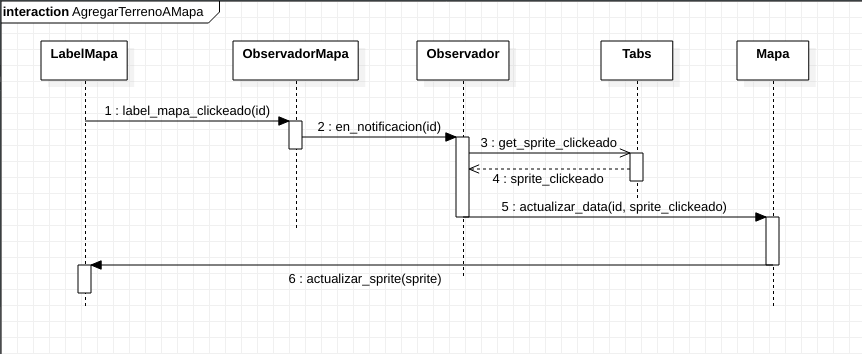
\includegraphics[width=0.8\textwidth]{../imagenes/seq_uml_agregar_terreno_editor.png}
	\caption{\label{fig:seq_uml_agregar_terreno} Diagrama de secuencia UML: agregar terreno al mapa.}
\end{figure}

\end{itemize}

\subsection{Descripción de archivos}

\begin{itemize}

\item Mapa\\

El Editor tiene la función de crear mapas y almacenarlos en memoria. Elegimos almacenarlos en el formato JSON por las razones indicadas en la 'Descripción general' del informe técnico en la sección del Editor. Dentro del archivo JSON se almacenas 2 arrays: uno representa la posicion de cada jugador en el mapa y el otro reprenta al mapa en si mismo. \\

El array de jugadores es de largo n siendo n la cantidad de jugadores. Cada elemento del array de jugadores a su vez es un array de largo 2 que representa la posición en el mapa del jugador, [X, Y]. \\

El array que representa al mapa también es una array de arrays. En este caso los arrays que se encuentran dentro del array principal son de largo k siendo k la cantidad de columnas del mapa y el array principal tiene un largo de h siendo h la cantidad de filas del mapa. Dentro de los arrays secundarios se ubican strings que representas los diferentes terrenos ubicables en el mapa. A continuación explicaremos que son esos strings en el item 'Sprites terrenos'.

\item Sprites terrenos\\

Los sprites de los terrenos están distribuidos en cuadrados de 8x8 pixeles en el archivo 'd2k\_BLOXBASE.bmp' cuyo tamaño es de 160x320 pixeles. A su vez cada tile del mapa tiene un tamaño de 32x32 pixeles, lo que serían 16 cuadrados de 8x8. A su vez cada tile tiene un id en formato string (por ejemplo: "arena1") y un tipo en formato int (por ejemplo: "0"). Para cada tipo de terreno existen distintos tiles con distintos ids (por ejemplo: "roca1", "roca2", étc.).\\

En el archivo terrenos.json se encuentran los distintos tipos de terrenos con sus respectivos tiles. Cada tile esta representado por un vector de ints de largo 16, cada elemento representa la posición de un cuadrado de 8x8 pixeles en el archivo .bmp indicado anteriormente, siendo el cuadrado que se encuentra en la esquina superior izquierda el 1, el cuadrado que se encuentra a su derecha el 2 y sigue contando de esa manera.

\item Editor.ui\\

Dicho archivo, editable con el programa Qt Designer, almacena la información de la interfaz gráfica (el diseño o wireframe, los distintos widgets, étc.).

\end{itemize}

\end{document}